\documentclass{standalone}%
\usepackage[T1]{fontenc}%
\usepackage[utf8]{inputenc}%
\usepackage{lmodern}%
\usepackage{textcomp}%
\usepackage{lastpage}%
\usepackage{tikz}%
%
%
%
\begin{document}%
\normalsize%
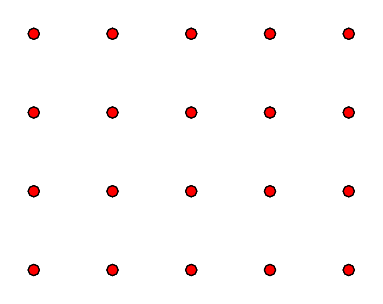
\begin{tikzpicture}[scale=1]%
\path[draw,radius=2pt,fill=red] (0.0,-5.0) circle;%
\path[draw,radius=2pt,fill=red] (1.0,-5.0) circle;%
\path[draw,radius=2pt,fill=red] (2.0,-5.0) circle;%
\path[draw,radius=2pt,fill=red] (3.0,-5.0) circle;%
\path[draw,radius=2pt,fill=red] (4.0,-5.0) circle;%
\path[draw,radius=2pt,fill=red] (0.0,-6.0) circle;%
\path[draw,radius=2pt,fill=red] (1.0,-6.0) circle;%
\path[draw,radius=2pt,fill=red] (2.0,-6.0) circle;%
\path[draw,radius=2pt,fill=red] (3.0,-6.0) circle;%
\path[draw,radius=2pt,fill=red] (4.0,-6.0) circle;%
\path[draw,radius=2pt,fill=red] (0.0,-7.0) circle;%
\path[draw,radius=2pt,fill=red] (1.0,-7.0) circle;%
\path[draw,radius=2pt,fill=red] (2.0,-7.0) circle;%
\path[draw,radius=2pt,fill=red] (3.0,-7.0) circle;%
\path[draw,radius=2pt,fill=red] (4.0,-7.0) circle;%
\path[draw,radius=2pt,fill=red] (0.0,-8.0) circle;%
\path[draw,radius=2pt,fill=red] (1.0,-8.0) circle;%
\path[draw,radius=2pt,fill=red] (2.0,-8.0) circle;%
\path[draw,radius=2pt,fill=red] (3.0,-8.0) circle;%
\path[draw,radius=2pt,fill=red] (4.0,-8.0) circle;%
\path[draw,radius=2pt,fill=red] (0.0,-5.0) circle;%
\path[draw,radius=2pt,fill=red] (1.0,-5.0) circle;%
\path[draw,radius=2pt,fill=red] (2.0,-5.0) circle;%
\path[draw,radius=2pt,fill=red] (3.0,-5.0) circle;%
\path[draw,radius=2pt,fill=red] (4.0,-5.0) circle;%
\path[draw,radius=2pt,fill=red] (0.0,-6.0) circle;%
\path[draw,radius=2pt,fill=red] (1.0,-6.0) circle;%
\path[draw,radius=2pt,fill=red] (2.0,-6.0) circle;%
\path[draw,radius=2pt,fill=red] (3.0,-6.0) circle;%
\path[draw,radius=2pt,fill=red] (4.0,-6.0) circle;%
\path[draw,radius=2pt,fill=red] (0.0,-7.0) circle;%
\path[draw,radius=2pt,fill=red] (1.0,-7.0) circle;%
\path[draw,radius=2pt,fill=red] (2.0,-7.0) circle;%
\path[draw,radius=2pt,fill=red] (3.0,-7.0) circle;%
\path[draw,radius=2pt,fill=red] (4.0,-7.0) circle;%
\path[draw,radius=2pt,fill=red] (0.0,-8.0) circle;%
\path[draw,radius=2pt,fill=red] (1.0,-8.0) circle;%
\path[draw,radius=2pt,fill=red] (2.0,-8.0) circle;%
\path[draw,radius=2pt,fill=red] (3.0,-8.0) circle;%
\path[draw,radius=2pt,fill=red] (4.0,-8.0) circle;%
\path[draw,radius=2pt,fill=red] (0.0,-5.0) circle;%
\path[draw,radius=2pt,fill=red] (1.0,-5.0) circle;%
\path[draw,radius=2pt,fill=red] (2.0,-5.0) circle;%
\path[draw,radius=2pt,fill=red] (3.0,-5.0) circle;%
\path[draw,radius=2pt,fill=red] (4.0,-5.0) circle;%
\path[draw,radius=2pt,fill=red] (0.0,-6.0) circle;%
\path[draw,radius=2pt,fill=red] (1.0,-6.0) circle;%
\path[draw,radius=2pt,fill=red] (2.0,-6.0) circle;%
\path[draw,radius=2pt,fill=red] (3.0,-6.0) circle;%
\path[draw,radius=2pt,fill=red] (4.0,-6.0) circle;%
\path[draw,radius=2pt,fill=red] (0.0,-7.0) circle;%
\path[draw,radius=2pt,fill=red] (1.0,-7.0) circle;%
\path[draw,radius=2pt,fill=red] (2.0,-7.0) circle;%
\path[draw,radius=2pt,fill=red] (3.0,-7.0) circle;%
\path[draw,radius=2pt,fill=red] (4.0,-7.0) circle;%
\path[draw,radius=2pt,fill=red] (0.0,-8.0) circle;%
\path[draw,radius=2pt,fill=red] (1.0,-8.0) circle;%
\path[draw,radius=2pt,fill=red] (2.0,-8.0) circle;%
\path[draw,radius=2pt,fill=red] (3.0,-8.0) circle;%
\path[draw,radius=2pt,fill=red] (4.0,-8.0) circle;%
\end{tikzpicture}%
\hspace*{1in}%
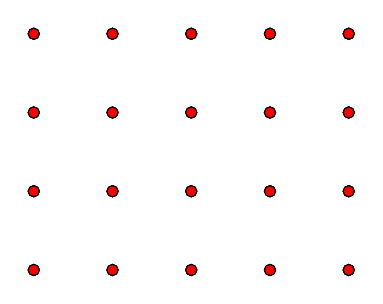
\begin{tikzpicture}[scale=1]%
\path[draw,radius=2pt] (4.0,-8.0) circle;%
\path[draw,radius=2pt,fill=red] (0.0,-5.0) circle;%
\path[draw,radius=2pt,fill=red] (1.0,-5.0) circle;%
\path[draw,radius=2pt,fill=red] (2.0,-5.0) circle;%
\path[draw,radius=2pt,fill=red] (3.0,-5.0) circle;%
\path[draw,radius=2pt,fill=red] (4.0,-5.0) circle;%
\path[draw,radius=2pt,fill=red] (0.0,-6.0) circle;%
\path[draw,radius=2pt,fill=red] (1.0,-6.0) circle;%
\path[draw,radius=2pt,fill=red] (2.0,-6.0) circle;%
\path[draw,radius=2pt,fill=red] (3.0,-6.0) circle;%
\path[draw,radius=2pt,fill=red] (4.0,-6.0) circle;%
\path[draw,radius=2pt,fill=red] (0.0,-7.0) circle;%
\path[draw,radius=2pt,fill=red] (1.0,-7.0) circle;%
\path[draw,radius=2pt,fill=red] (2.0,-7.0) circle;%
\path[draw,radius=2pt,fill=red] (3.0,-7.0) circle;%
\path[draw,radius=2pt,fill=red] (4.0,-7.0) circle;%
\path[draw,radius=2pt,fill=red] (0.0,-8.0) circle;%
\path[draw,radius=2pt,fill=red] (1.0,-8.0) circle;%
\path[draw,radius=2pt,fill=red] (2.0,-8.0) circle;%
\path[draw,radius=2pt,fill=red] (3.0,-8.0) circle;%
\path[draw,radius=2pt,fill=red] (4.0,-8.0) circle;%
\path[draw,radius=2pt,fill=red] (0.0,-5.0) circle;%
\path[draw,radius=2pt,fill=red] (1.0,-5.0) circle;%
\path[draw,radius=2pt,fill=red] (2.0,-5.0) circle;%
\path[draw,radius=2pt,fill=red] (3.0,-5.0) circle;%
\path[draw,radius=2pt,fill=red] (4.0,-5.0) circle;%
\path[draw,radius=2pt,fill=red] (0.0,-6.0) circle;%
\path[draw,radius=2pt,fill=red] (1.0,-6.0) circle;%
\path[draw,radius=2pt,fill=red] (2.0,-6.0) circle;%
\path[draw,radius=2pt,fill=red] (3.0,-6.0) circle;%
\path[draw,radius=2pt,fill=red] (4.0,-6.0) circle;%
\path[draw,radius=2pt,fill=red] (0.0,-7.0) circle;%
\path[draw,radius=2pt,fill=red] (1.0,-7.0) circle;%
\path[draw,radius=2pt,fill=red] (2.0,-7.0) circle;%
\path[draw,radius=2pt,fill=red] (3.0,-7.0) circle;%
\path[draw,radius=2pt,fill=red] (4.0,-7.0) circle;%
\path[draw,radius=2pt,fill=red] (0.0,-8.0) circle;%
\path[draw,radius=2pt,fill=red] (1.0,-8.0) circle;%
\path[draw,radius=2pt,fill=red] (2.0,-8.0) circle;%
\path[draw,radius=2pt,fill=red] (3.0,-8.0) circle;%
\path[draw,radius=2pt,fill=red] (4.0,-8.0) circle;%
\path[draw,radius=2pt,fill=red] (0.0,-5.0) circle;%
\path[draw,radius=2pt,fill=red] (1.0,-5.0) circle;%
\path[draw,radius=2pt,fill=red] (2.0,-5.0) circle;%
\path[draw,radius=2pt,fill=red] (3.0,-5.0) circle;%
\path[draw,radius=2pt,fill=red] (4.0,-5.0) circle;%
\path[draw,radius=2pt,fill=red] (0.0,-6.0) circle;%
\path[draw,radius=2pt,fill=red] (1.0,-6.0) circle;%
\path[draw,radius=2pt,fill=red] (2.0,-6.0) circle;%
\path[draw,radius=2pt,fill=red] (3.0,-6.0) circle;%
\path[draw,radius=2pt,fill=red] (4.0,-6.0) circle;%
\path[draw,radius=2pt,fill=red] (0.0,-7.0) circle;%
\path[draw,radius=2pt,fill=red] (1.0,-7.0) circle;%
\path[draw,radius=2pt,fill=red] (2.0,-7.0) circle;%
\path[draw,radius=2pt,fill=red] (3.0,-7.0) circle;%
\path[draw,radius=2pt,fill=red] (4.0,-7.0) circle;%
\path[draw,radius=2pt,fill=red] (0.0,-8.0) circle;%
\path[draw,radius=2pt,fill=red] (1.0,-8.0) circle;%
\path[draw,radius=2pt,fill=red] (2.0,-8.0) circle;%
\path[draw,radius=2pt,fill=red] (3.0,-8.0) circle;%
\end{tikzpicture}%
\hspace*{1in}%
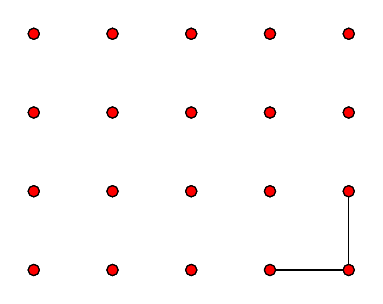
\begin{tikzpicture}[scale=1]%
\path[draw,radius=2pt] (0.0,-5.0) circle;%
\path[draw] (4.0,-7.0) -- (4.0,-8.0);%
\path[draw,radius=2pt] (4.0,-7.0) circle;%
\path[draw] (3.0,-8.0) -- (4.0,-8.0);%
\path[draw,radius=2pt] (3.0,-8.0) circle;%
\path[draw] (4.0,-8.0) -- (4.0,-7.0);%
\path[draw] (4.0,-8.0) -- (3.0,-8.0);%
\path[draw,radius=2pt] (4.0,-8.0) circle;%
\path[draw,radius=2pt,fill=red] (0.0,-5.0) circle;%
\path[draw,radius=2pt,fill=red] (1.0,-5.0) circle;%
\path[draw,radius=2pt,fill=red] (2.0,-5.0) circle;%
\path[draw,radius=2pt,fill=red] (3.0,-5.0) circle;%
\path[draw,radius=2pt,fill=red] (4.0,-5.0) circle;%
\path[draw,radius=2pt,fill=red] (0.0,-6.0) circle;%
\path[draw,radius=2pt,fill=red] (1.0,-6.0) circle;%
\path[draw,radius=2pt,fill=red] (2.0,-6.0) circle;%
\path[draw,radius=2pt,fill=red] (3.0,-6.0) circle;%
\path[draw,radius=2pt,fill=red] (4.0,-6.0) circle;%
\path[draw,radius=2pt,fill=red] (0.0,-7.0) circle;%
\path[draw,radius=2pt,fill=red] (1.0,-7.0) circle;%
\path[draw,radius=2pt,fill=red] (2.0,-7.0) circle;%
\path[draw,radius=2pt,fill=red] (3.0,-7.0) circle;%
\path[draw,radius=2pt,fill=red] (4.0,-7.0) circle;%
\path[draw,radius=2pt,fill=red] (0.0,-8.0) circle;%
\path[draw,radius=2pt,fill=red] (1.0,-8.0) circle;%
\path[draw,radius=2pt,fill=red] (2.0,-8.0) circle;%
\path[draw,radius=2pt,fill=red] (3.0,-8.0) circle;%
\path[draw,radius=2pt,fill=red] (4.0,-8.0) circle;%
\path[draw,radius=2pt,fill=red] (0.0,-5.0) circle;%
\path[draw,radius=2pt,fill=red] (1.0,-5.0) circle;%
\path[draw,radius=2pt,fill=red] (2.0,-5.0) circle;%
\path[draw,radius=2pt,fill=red] (3.0,-5.0) circle;%
\path[draw,radius=2pt,fill=red] (4.0,-5.0) circle;%
\path[draw,radius=2pt,fill=red] (0.0,-6.0) circle;%
\path[draw,radius=2pt,fill=red] (1.0,-6.0) circle;%
\path[draw,radius=2pt,fill=red] (2.0,-6.0) circle;%
\path[draw,radius=2pt,fill=red] (3.0,-6.0) circle;%
\path[draw,radius=2pt,fill=red] (4.0,-6.0) circle;%
\path[draw,radius=2pt,fill=red] (0.0,-7.0) circle;%
\path[draw,radius=2pt,fill=red] (1.0,-7.0) circle;%
\path[draw,radius=2pt,fill=red] (2.0,-7.0) circle;%
\path[draw,radius=2pt,fill=red] (3.0,-7.0) circle;%
\path[draw,radius=2pt,fill=red] (4.0,-7.0) circle;%
\path[draw,radius=2pt,fill=red] (0.0,-8.0) circle;%
\path[draw,radius=2pt,fill=red] (1.0,-8.0) circle;%
\path[draw,radius=2pt,fill=red] (2.0,-8.0) circle;%
\path[draw,radius=2pt,fill=red] (3.0,-8.0) circle;%
\path[draw,radius=2pt,fill=red] (4.0,-8.0) circle;%
\path[draw,radius=2pt,fill=red] (1.0,-5.0) circle;%
\path[draw,radius=2pt,fill=red] (2.0,-5.0) circle;%
\path[draw,radius=2pt,fill=red] (3.0,-5.0) circle;%
\path[draw,radius=2pt,fill=red] (4.0,-5.0) circle;%
\path[draw,radius=2pt,fill=red] (0.0,-6.0) circle;%
\path[draw,radius=2pt,fill=red] (1.0,-6.0) circle;%
\path[draw,radius=2pt,fill=red] (2.0,-6.0) circle;%
\path[draw,radius=2pt,fill=red] (3.0,-6.0) circle;%
\path[draw,radius=2pt,fill=red] (4.0,-6.0) circle;%
\path[draw,radius=2pt,fill=red] (0.0,-7.0) circle;%
\path[draw,radius=2pt,fill=red] (1.0,-7.0) circle;%
\path[draw,radius=2pt,fill=red] (2.0,-7.0) circle;%
\path[draw,radius=2pt,fill=red] (3.0,-7.0) circle;%
\path[draw,radius=2pt,fill=red] (0.0,-8.0) circle;%
\path[draw,radius=2pt,fill=red] (1.0,-8.0) circle;%
\path[draw,radius=2pt,fill=red] (2.0,-8.0) circle;%
\end{tikzpicture}%
\hspace*{1in}%
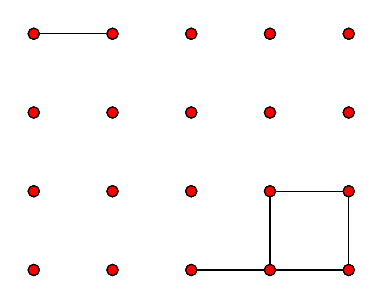
\begin{tikzpicture}[scale=1]%
\path[draw,radius=2pt] (2.0,-8.0) circle;%
\path[draw] (0.0,-5.0) -- (1.0,-5.0);%
\path[draw,radius=2pt] (0.0,-5.0) circle;%
\path[draw] (1.0,-5.0) -- (0.0,-5.0);%
\path[draw,radius=2pt] (1.0,-5.0) circle;%
\path[draw] (3.0,-7.0) -- (3.0,-8.0);%
\path[draw] (3.0,-7.0) -- (4.0,-7.0);%
\path[draw,radius=2pt] (3.0,-7.0) circle;%
\path[draw] (4.0,-7.0) -- (4.0,-8.0);%
\path[draw] (4.0,-7.0) -- (3.0,-7.0);%
\path[draw,radius=2pt] (4.0,-7.0) circle;%
\path[draw] (2.0,-8.0) -- (3.0,-8.0);%
\path[draw,radius=2pt] (2.0,-8.0) circle;%
\path[draw] (3.0,-8.0) -- (3.0,-7.0);%
\path[draw] (3.0,-8.0) -- (2.0,-8.0);%
\path[draw] (3.0,-8.0) -- (4.0,-8.0);%
\path[draw,radius=2pt] (3.0,-8.0) circle;%
\path[draw] (4.0,-8.0) -- (4.0,-7.0);%
\path[draw] (4.0,-8.0) -- (3.0,-8.0);%
\path[draw,radius=2pt] (4.0,-8.0) circle;%
\path[draw,radius=2pt,fill=red] (0.0,-5.0) circle;%
\path[draw,radius=2pt,fill=red] (1.0,-5.0) circle;%
\path[draw,radius=2pt,fill=red] (2.0,-5.0) circle;%
\path[draw,radius=2pt,fill=red] (3.0,-5.0) circle;%
\path[draw,radius=2pt,fill=red] (4.0,-5.0) circle;%
\path[draw,radius=2pt,fill=red] (0.0,-6.0) circle;%
\path[draw,radius=2pt,fill=red] (1.0,-6.0) circle;%
\path[draw,radius=2pt,fill=red] (2.0,-6.0) circle;%
\path[draw,radius=2pt,fill=red] (3.0,-6.0) circle;%
\path[draw,radius=2pt,fill=red] (4.0,-6.0) circle;%
\path[draw,radius=2pt,fill=red] (0.0,-7.0) circle;%
\path[draw,radius=2pt,fill=red] (1.0,-7.0) circle;%
\path[draw,radius=2pt,fill=red] (2.0,-7.0) circle;%
\path[draw,radius=2pt,fill=red] (3.0,-7.0) circle;%
\path[draw,radius=2pt,fill=red] (4.0,-7.0) circle;%
\path[draw,radius=2pt,fill=red] (0.0,-8.0) circle;%
\path[draw,radius=2pt,fill=red] (1.0,-8.0) circle;%
\path[draw,radius=2pt,fill=red] (3.0,-8.0) circle;%
\path[draw,radius=2pt,fill=red] (4.0,-8.0) circle;%
\path[draw,radius=2pt,fill=red] (0.0,-5.0) circle;%
\path[draw,radius=2pt,fill=red] (1.0,-5.0) circle;%
\path[draw,radius=2pt,fill=red] (2.0,-5.0) circle;%
\path[draw,radius=2pt,fill=red] (3.0,-5.0) circle;%
\path[draw,radius=2pt,fill=red] (4.0,-5.0) circle;%
\path[draw,radius=2pt,fill=red] (0.0,-6.0) circle;%
\path[draw,radius=2pt,fill=red] (1.0,-6.0) circle;%
\path[draw,radius=2pt,fill=red] (2.0,-6.0) circle;%
\path[draw,radius=2pt,fill=red] (3.0,-6.0) circle;%
\path[draw,radius=2pt,fill=red] (4.0,-6.0) circle;%
\path[draw,radius=2pt,fill=red] (0.0,-7.0) circle;%
\path[draw,radius=2pt,fill=red] (1.0,-7.0) circle;%
\path[draw,radius=2pt,fill=red] (2.0,-7.0) circle;%
\path[draw,radius=2pt,fill=red] (3.0,-7.0) circle;%
\path[draw,radius=2pt,fill=red] (4.0,-7.0) circle;%
\path[draw,radius=2pt,fill=red] (0.0,-8.0) circle;%
\path[draw,radius=2pt,fill=red] (1.0,-8.0) circle;%
\path[draw,radius=2pt,fill=red] (2.0,-8.0) circle;%
\path[draw,radius=2pt,fill=red] (3.0,-8.0) circle;%
\path[draw,radius=2pt,fill=red] (4.0,-8.0) circle;%
\path[draw,radius=2pt,fill=red] (2.0,-5.0) circle;%
\path[draw,radius=2pt,fill=red] (3.0,-5.0) circle;%
\path[draw,radius=2pt,fill=red] (4.0,-5.0) circle;%
\path[draw,radius=2pt,fill=red] (0.0,-6.0) circle;%
\path[draw,radius=2pt,fill=red] (1.0,-6.0) circle;%
\path[draw,radius=2pt,fill=red] (2.0,-6.0) circle;%
\path[draw,radius=2pt,fill=red] (3.0,-6.0) circle;%
\path[draw,radius=2pt,fill=red] (4.0,-6.0) circle;%
\path[draw,radius=2pt,fill=red] (0.0,-7.0) circle;%
\path[draw,radius=2pt,fill=red] (1.0,-7.0) circle;%
\path[draw,radius=2pt,fill=red] (2.0,-7.0) circle;%
\path[draw,radius=2pt,fill=red] (0.0,-8.0) circle;%
\path[draw,radius=2pt,fill=red] (1.0,-8.0) circle;%
\end{tikzpicture}%
\newline%
\hspace*{1in}%
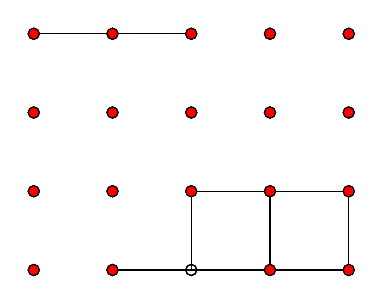
\begin{tikzpicture}[scale=1]%
\path[draw] (2.0,-7.0) -- (2.0,-8.0);%
\path[draw,radius=2pt] (2.0,-7.0) circle;%
\path[draw] (1.0,-8.0) -- (2.0,-8.0);%
\path[draw,radius=2pt] (1.0,-8.0) circle;%
\path[draw] (2.0,-8.0) -- (2.0,-7.0);%
\path[draw] (2.0,-8.0) -- (1.0,-8.0);%
\path[draw,radius=2pt] (2.0,-8.0) circle;%
\path[draw,radius=2pt] (2.0,-8.0) circle;%
\path[draw] (0.0,-5.0) -- (1.0,-5.0);%
\path[draw,radius=2pt] (0.0,-5.0) circle;%
\path[draw] (1.0,-5.0) -- (0.0,-5.0);%
\path[draw] (1.0,-5.0) -- (2.0,-5.0);%
\path[draw,radius=2pt] (1.0,-5.0) circle;%
\path[draw] (2.0,-5.0) -- (1.0,-5.0);%
\path[draw,radius=2pt] (2.0,-5.0) circle;%
\path[draw] (2.0,-7.0) -- (2.0,-8.0);%
\path[draw] (2.0,-7.0) -- (3.0,-7.0);%
\path[draw,radius=2pt] (2.0,-7.0) circle;%
\path[draw] (3.0,-7.0) -- (3.0,-8.0);%
\path[draw] (3.0,-7.0) -- (2.0,-7.0);%
\path[draw] (3.0,-7.0) -- (4.0,-7.0);%
\path[draw,radius=2pt] (3.0,-7.0) circle;%
\path[draw] (4.0,-7.0) -- (4.0,-8.0);%
\path[draw] (4.0,-7.0) -- (3.0,-7.0);%
\path[draw,radius=2pt] (4.0,-7.0) circle;%
\path[draw] (2.0,-8.0) -- (2.0,-7.0);%
\path[draw] (2.0,-8.0) -- (3.0,-8.0);%
\path[draw,radius=2pt] (2.0,-8.0) circle;%
\path[draw] (3.0,-8.0) -- (3.0,-7.0);%
\path[draw] (3.0,-8.0) -- (2.0,-8.0);%
\path[draw] (3.0,-8.0) -- (4.0,-8.0);%
\path[draw,radius=2pt] (3.0,-8.0) circle;%
\path[draw] (4.0,-8.0) -- (4.0,-7.0);%
\path[draw] (4.0,-8.0) -- (3.0,-8.0);%
\path[draw,radius=2pt] (4.0,-8.0) circle;%
\path[draw,radius=2pt,fill=red] (0.0,-5.0) circle;%
\path[draw,radius=2pt,fill=red] (1.0,-5.0) circle;%
\path[draw,radius=2pt,fill=red] (2.0,-5.0) circle;%
\path[draw,radius=2pt,fill=red] (3.0,-5.0) circle;%
\path[draw,radius=2pt,fill=red] (4.0,-5.0) circle;%
\path[draw,radius=2pt,fill=red] (0.0,-6.0) circle;%
\path[draw,radius=2pt,fill=red] (1.0,-6.0) circle;%
\path[draw,radius=2pt,fill=red] (2.0,-6.0) circle;%
\path[draw,radius=2pt,fill=red] (3.0,-6.0) circle;%
\path[draw,radius=2pt,fill=red] (4.0,-6.0) circle;%
\path[draw,radius=2pt,fill=red] (0.0,-7.0) circle;%
\path[draw,radius=2pt,fill=red] (1.0,-7.0) circle;%
\path[draw,radius=2pt,fill=red] (3.0,-7.0) circle;%
\path[draw,radius=2pt,fill=red] (4.0,-7.0) circle;%
\path[draw,radius=2pt,fill=red] (0.0,-8.0) circle;%
\path[draw,radius=2pt,fill=red] (3.0,-8.0) circle;%
\path[draw,radius=2pt,fill=red] (4.0,-8.0) circle;%
\path[draw,radius=2pt,fill=red] (0.0,-5.0) circle;%
\path[draw,radius=2pt,fill=red] (1.0,-5.0) circle;%
\path[draw,radius=2pt,fill=red] (2.0,-5.0) circle;%
\path[draw,radius=2pt,fill=red] (3.0,-5.0) circle;%
\path[draw,radius=2pt,fill=red] (4.0,-5.0) circle;%
\path[draw,radius=2pt,fill=red] (0.0,-6.0) circle;%
\path[draw,radius=2pt,fill=red] (1.0,-6.0) circle;%
\path[draw,radius=2pt,fill=red] (2.0,-6.0) circle;%
\path[draw,radius=2pt,fill=red] (3.0,-6.0) circle;%
\path[draw,radius=2pt,fill=red] (4.0,-6.0) circle;%
\path[draw,radius=2pt,fill=red] (0.0,-7.0) circle;%
\path[draw,radius=2pt,fill=red] (1.0,-7.0) circle;%
\path[draw,radius=2pt,fill=red] (2.0,-7.0) circle;%
\path[draw,radius=2pt,fill=red] (3.0,-7.0) circle;%
\path[draw,radius=2pt,fill=red] (4.0,-7.0) circle;%
\path[draw,radius=2pt,fill=red] (0.0,-8.0) circle;%
\path[draw,radius=2pt,fill=red] (1.0,-8.0) circle;%
\path[draw,radius=2pt,fill=red] (3.0,-8.0) circle;%
\path[draw,radius=2pt,fill=red] (4.0,-8.0) circle;%
\path[draw,radius=2pt,fill=red] (3.0,-5.0) circle;%
\path[draw,radius=2pt,fill=red] (4.0,-5.0) circle;%
\path[draw,radius=2pt,fill=red] (0.0,-6.0) circle;%
\path[draw,radius=2pt,fill=red] (1.0,-6.0) circle;%
\path[draw,radius=2pt,fill=red] (2.0,-6.0) circle;%
\path[draw,radius=2pt,fill=red] (3.0,-6.0) circle;%
\path[draw,radius=2pt,fill=red] (4.0,-6.0) circle;%
\path[draw,radius=2pt,fill=red] (0.0,-7.0) circle;%
\path[draw,radius=2pt,fill=red] (1.0,-7.0) circle;%
\path[draw,radius=2pt,fill=red] (0.0,-8.0) circle;%
\path[draw,radius=2pt,fill=red] (1.0,-8.0) circle;%
\end{tikzpicture}%
\hspace*{1in}%
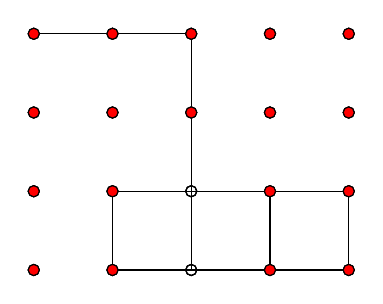
\begin{tikzpicture}[scale=1]%
\path[draw] (2.0,-6.0) -- (2.0,-7.0);%
\path[draw,radius=2pt] (2.0,-6.0) circle;%
\path[draw] (1.0,-7.0) -- (1.0,-8.0);%
\path[draw] (1.0,-7.0) -- (2.0,-7.0);%
\path[draw,radius=2pt] (1.0,-7.0) circle;%
\path[draw] (2.0,-7.0) -- (2.0,-6.0);%
\path[draw] (2.0,-7.0) -- (2.0,-8.0);%
\path[draw] (2.0,-7.0) -- (1.0,-7.0);%
\path[draw,radius=2pt] (2.0,-7.0) circle;%
\path[draw] (1.0,-8.0) -- (1.0,-7.0);%
\path[draw] (1.0,-8.0) -- (2.0,-8.0);%
\path[draw,radius=2pt] (1.0,-8.0) circle;%
\path[draw] (2.0,-8.0) -- (2.0,-7.0);%
\path[draw] (2.0,-8.0) -- (1.0,-8.0);%
\path[draw,radius=2pt] (2.0,-8.0) circle;%
\path[draw] (2.0,-7.0) -- (2.0,-8.0);%
\path[draw,radius=2pt] (2.0,-7.0) circle;%
\path[draw] (2.0,-8.0) -- (2.0,-7.0);%
\path[draw,radius=2pt] (2.0,-8.0) circle;%
\path[draw] (0.0,-5.0) -- (1.0,-5.0);%
\path[draw,radius=2pt] (0.0,-5.0) circle;%
\path[draw] (1.0,-5.0) -- (0.0,-5.0);%
\path[draw] (1.0,-5.0) -- (2.0,-5.0);%
\path[draw,radius=2pt] (1.0,-5.0) circle;%
\path[draw] (2.0,-5.0) -- (2.0,-6.0);%
\path[draw] (2.0,-5.0) -- (1.0,-5.0);%
\path[draw,radius=2pt] (2.0,-5.0) circle;%
\path[draw] (2.0,-6.0) -- (2.0,-5.0);%
\path[draw] (2.0,-6.0) -- (2.0,-7.0);%
\path[draw,radius=2pt] (2.0,-6.0) circle;%
\path[draw] (2.0,-7.0) -- (2.0,-6.0);%
\path[draw] (2.0,-7.0) -- (2.0,-8.0);%
\path[draw] (2.0,-7.0) -- (3.0,-7.0);%
\path[draw,radius=2pt] (2.0,-7.0) circle;%
\path[draw] (3.0,-7.0) -- (3.0,-8.0);%
\path[draw] (3.0,-7.0) -- (2.0,-7.0);%
\path[draw] (3.0,-7.0) -- (4.0,-7.0);%
\path[draw,radius=2pt] (3.0,-7.0) circle;%
\path[draw] (4.0,-7.0) -- (4.0,-8.0);%
\path[draw] (4.0,-7.0) -- (3.0,-7.0);%
\path[draw,radius=2pt] (4.0,-7.0) circle;%
\path[draw] (2.0,-8.0) -- (2.0,-7.0);%
\path[draw] (2.0,-8.0) -- (3.0,-8.0);%
\path[draw,radius=2pt] (2.0,-8.0) circle;%
\path[draw] (3.0,-8.0) -- (3.0,-7.0);%
\path[draw] (3.0,-8.0) -- (2.0,-8.0);%
\path[draw] (3.0,-8.0) -- (4.0,-8.0);%
\path[draw,radius=2pt] (3.0,-8.0) circle;%
\path[draw] (4.0,-8.0) -- (4.0,-7.0);%
\path[draw] (4.0,-8.0) -- (3.0,-8.0);%
\path[draw,radius=2pt] (4.0,-8.0) circle;%
\path[draw,radius=2pt,fill=red] (0.0,-5.0) circle;%
\path[draw,radius=2pt,fill=red] (1.0,-5.0) circle;%
\path[draw,radius=2pt,fill=red] (2.0,-5.0) circle;%
\path[draw,radius=2pt,fill=red] (3.0,-5.0) circle;%
\path[draw,radius=2pt,fill=red] (4.0,-5.0) circle;%
\path[draw,radius=2pt,fill=red] (0.0,-6.0) circle;%
\path[draw,radius=2pt,fill=red] (1.0,-6.0) circle;%
\path[draw,radius=2pt,fill=red] (3.0,-6.0) circle;%
\path[draw,radius=2pt,fill=red] (4.0,-6.0) circle;%
\path[draw,radius=2pt,fill=red] (0.0,-7.0) circle;%
\path[draw,radius=2pt,fill=red] (3.0,-7.0) circle;%
\path[draw,radius=2pt,fill=red] (4.0,-7.0) circle;%
\path[draw,radius=2pt,fill=red] (0.0,-8.0) circle;%
\path[draw,radius=2pt,fill=red] (3.0,-8.0) circle;%
\path[draw,radius=2pt,fill=red] (4.0,-8.0) circle;%
\path[draw,radius=2pt,fill=red] (0.0,-5.0) circle;%
\path[draw,radius=2pt,fill=red] (1.0,-5.0) circle;%
\path[draw,radius=2pt,fill=red] (2.0,-5.0) circle;%
\path[draw,radius=2pt,fill=red] (3.0,-5.0) circle;%
\path[draw,radius=2pt,fill=red] (4.0,-5.0) circle;%
\path[draw,radius=2pt,fill=red] (0.0,-6.0) circle;%
\path[draw,radius=2pt,fill=red] (1.0,-6.0) circle;%
\path[draw,radius=2pt,fill=red] (2.0,-6.0) circle;%
\path[draw,radius=2pt,fill=red] (3.0,-6.0) circle;%
\path[draw,radius=2pt,fill=red] (4.0,-6.0) circle;%
\path[draw,radius=2pt,fill=red] (0.0,-7.0) circle;%
\path[draw,radius=2pt,fill=red] (1.0,-7.0) circle;%
\path[draw,radius=2pt,fill=red] (3.0,-7.0) circle;%
\path[draw,radius=2pt,fill=red] (4.0,-7.0) circle;%
\path[draw,radius=2pt,fill=red] (0.0,-8.0) circle;%
\path[draw,radius=2pt,fill=red] (1.0,-8.0) circle;%
\path[draw,radius=2pt,fill=red] (3.0,-8.0) circle;%
\path[draw,radius=2pt,fill=red] (4.0,-8.0) circle;%
\path[draw,radius=2pt,fill=red] (3.0,-5.0) circle;%
\path[draw,radius=2pt,fill=red] (4.0,-5.0) circle;%
\path[draw,radius=2pt,fill=red] (0.0,-6.0) circle;%
\path[draw,radius=2pt,fill=red] (1.0,-6.0) circle;%
\path[draw,radius=2pt,fill=red] (3.0,-6.0) circle;%
\path[draw,radius=2pt,fill=red] (4.0,-6.0) circle;%
\path[draw,radius=2pt,fill=red] (0.0,-7.0) circle;%
\path[draw,radius=2pt,fill=red] (1.0,-7.0) circle;%
\path[draw,radius=2pt,fill=red] (0.0,-8.0) circle;%
\path[draw,radius=2pt,fill=red] (1.0,-8.0) circle;%
\end{tikzpicture}%
\hspace*{1in}%
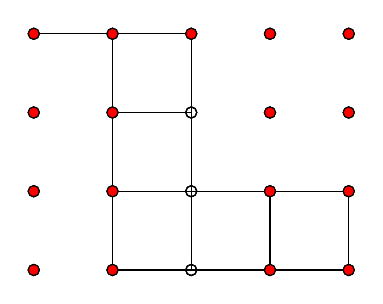
\begin{tikzpicture}[scale=1]%
\path[draw] (1.0,-6.0) -- (1.0,-7.0);%
\path[draw] (1.0,-6.0) -- (2.0,-6.0);%
\path[draw,radius=2pt] (1.0,-6.0) circle;%
\path[draw] (2.0,-6.0) -- (2.0,-7.0);%
\path[draw] (2.0,-6.0) -- (1.0,-6.0);%
\path[draw,radius=2pt] (2.0,-6.0) circle;%
\path[draw] (1.0,-7.0) -- (1.0,-6.0);%
\path[draw] (1.0,-7.0) -- (1.0,-8.0);%
\path[draw] (1.0,-7.0) -- (2.0,-7.0);%
\path[draw,radius=2pt] (1.0,-7.0) circle;%
\path[draw] (2.0,-7.0) -- (2.0,-6.0);%
\path[draw] (2.0,-7.0) -- (2.0,-8.0);%
\path[draw] (2.0,-7.0) -- (1.0,-7.0);%
\path[draw,radius=2pt] (2.0,-7.0) circle;%
\path[draw] (1.0,-8.0) -- (1.0,-7.0);%
\path[draw] (1.0,-8.0) -- (2.0,-8.0);%
\path[draw,radius=2pt] (1.0,-8.0) circle;%
\path[draw] (2.0,-8.0) -- (2.0,-7.0);%
\path[draw] (2.0,-8.0) -- (1.0,-8.0);%
\path[draw,radius=2pt] (2.0,-8.0) circle;%
\path[draw] (2.0,-6.0) -- (2.0,-7.0);%
\path[draw,radius=2pt] (2.0,-6.0) circle;%
\path[draw] (2.0,-7.0) -- (2.0,-6.0);%
\path[draw] (2.0,-7.0) -- (2.0,-8.0);%
\path[draw,radius=2pt] (2.0,-7.0) circle;%
\path[draw] (2.0,-8.0) -- (2.0,-7.0);%
\path[draw,radius=2pt] (2.0,-8.0) circle;%
\path[draw,radius=2pt] (4.0,-8.0) circle;%
\path[draw] (0.0,-5.0) -- (1.0,-5.0);%
\path[draw,radius=2pt] (0.0,-5.0) circle;%
\path[draw] (1.0,-5.0) -- (1.0,-6.0);%
\path[draw] (1.0,-5.0) -- (0.0,-5.0);%
\path[draw] (1.0,-5.0) -- (2.0,-5.0);%
\path[draw,radius=2pt] (1.0,-5.0) circle;%
\path[draw] (2.0,-5.0) -- (2.0,-6.0);%
\path[draw] (2.0,-5.0) -- (1.0,-5.0);%
\path[draw,radius=2pt] (2.0,-5.0) circle;%
\path[draw] (1.0,-6.0) -- (1.0,-5.0);%
\path[draw] (1.0,-6.0) -- (2.0,-6.0);%
\path[draw,radius=2pt] (1.0,-6.0) circle;%
\path[draw] (2.0,-6.0) -- (2.0,-5.0);%
\path[draw] (2.0,-6.0) -- (2.0,-7.0);%
\path[draw] (2.0,-6.0) -- (1.0,-6.0);%
\path[draw,radius=2pt] (2.0,-6.0) circle;%
\path[draw] (2.0,-7.0) -- (2.0,-6.0);%
\path[draw] (2.0,-7.0) -- (2.0,-8.0);%
\path[draw] (2.0,-7.0) -- (3.0,-7.0);%
\path[draw,radius=2pt] (2.0,-7.0) circle;%
\path[draw] (3.0,-7.0) -- (3.0,-8.0);%
\path[draw] (3.0,-7.0) -- (2.0,-7.0);%
\path[draw] (3.0,-7.0) -- (4.0,-7.0);%
\path[draw,radius=2pt] (3.0,-7.0) circle;%
\path[draw] (4.0,-7.0) -- (4.0,-8.0);%
\path[draw] (4.0,-7.0) -- (3.0,-7.0);%
\path[draw,radius=2pt] (4.0,-7.0) circle;%
\path[draw] (2.0,-8.0) -- (2.0,-7.0);%
\path[draw] (2.0,-8.0) -- (3.0,-8.0);%
\path[draw,radius=2pt] (2.0,-8.0) circle;%
\path[draw] (3.0,-8.0) -- (3.0,-7.0);%
\path[draw] (3.0,-8.0) -- (2.0,-8.0);%
\path[draw] (3.0,-8.0) -- (4.0,-8.0);%
\path[draw,radius=2pt] (3.0,-8.0) circle;%
\path[draw] (4.0,-8.0) -- (4.0,-7.0);%
\path[draw] (4.0,-8.0) -- (3.0,-8.0);%
\path[draw,radius=2pt] (4.0,-8.0) circle;%
\path[draw,radius=2pt,fill=red] (0.0,-5.0) circle;%
\path[draw,radius=2pt,fill=red] (1.0,-5.0) circle;%
\path[draw,radius=2pt,fill=red] (2.0,-5.0) circle;%
\path[draw,radius=2pt,fill=red] (3.0,-5.0) circle;%
\path[draw,radius=2pt,fill=red] (4.0,-5.0) circle;%
\path[draw,radius=2pt,fill=red] (0.0,-6.0) circle;%
\path[draw,radius=2pt,fill=red] (3.0,-6.0) circle;%
\path[draw,radius=2pt,fill=red] (4.0,-6.0) circle;%
\path[draw,radius=2pt,fill=red] (0.0,-7.0) circle;%
\path[draw,radius=2pt,fill=red] (3.0,-7.0) circle;%
\path[draw,radius=2pt,fill=red] (4.0,-7.0) circle;%
\path[draw,radius=2pt,fill=red] (0.0,-8.0) circle;%
\path[draw,radius=2pt,fill=red] (3.0,-8.0) circle;%
\path[draw,radius=2pt,fill=red] (4.0,-8.0) circle;%
\path[draw,radius=2pt,fill=red] (0.0,-5.0) circle;%
\path[draw,radius=2pt,fill=red] (1.0,-5.0) circle;%
\path[draw,radius=2pt,fill=red] (2.0,-5.0) circle;%
\path[draw,radius=2pt,fill=red] (3.0,-5.0) circle;%
\path[draw,radius=2pt,fill=red] (4.0,-5.0) circle;%
\path[draw,radius=2pt,fill=red] (0.0,-6.0) circle;%
\path[draw,radius=2pt,fill=red] (1.0,-6.0) circle;%
\path[draw,radius=2pt,fill=red] (3.0,-6.0) circle;%
\path[draw,radius=2pt,fill=red] (4.0,-6.0) circle;%
\path[draw,radius=2pt,fill=red] (0.0,-7.0) circle;%
\path[draw,radius=2pt,fill=red] (1.0,-7.0) circle;%
\path[draw,radius=2pt,fill=red] (3.0,-7.0) circle;%
\path[draw,radius=2pt,fill=red] (4.0,-7.0) circle;%
\path[draw,radius=2pt,fill=red] (0.0,-8.0) circle;%
\path[draw,radius=2pt,fill=red] (1.0,-8.0) circle;%
\path[draw,radius=2pt,fill=red] (3.0,-8.0) circle;%
\path[draw,radius=2pt,fill=red] (3.0,-5.0) circle;%
\path[draw,radius=2pt,fill=red] (4.0,-5.0) circle;%
\path[draw,radius=2pt,fill=red] (0.0,-6.0) circle;%
\path[draw,radius=2pt,fill=red] (3.0,-6.0) circle;%
\path[draw,radius=2pt,fill=red] (4.0,-6.0) circle;%
\path[draw,radius=2pt,fill=red] (0.0,-7.0) circle;%
\path[draw,radius=2pt,fill=red] (1.0,-7.0) circle;%
\path[draw,radius=2pt,fill=red] (0.0,-8.0) circle;%
\path[draw,radius=2pt,fill=red] (1.0,-8.0) circle;%
\end{tikzpicture}%
\hspace*{1in}%
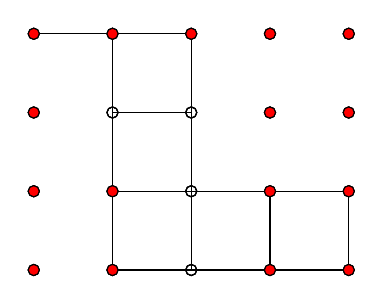
\begin{tikzpicture}[scale=1]%
\path[draw] (1.0,-6.0) -- (1.0,-7.0);%
\path[draw] (1.0,-6.0) -- (2.0,-6.0);%
\path[draw,radius=2pt] (1.0,-6.0) circle;%
\path[draw] (2.0,-6.0) -- (2.0,-7.0);%
\path[draw] (2.0,-6.0) -- (1.0,-6.0);%
\path[draw,radius=2pt] (2.0,-6.0) circle;%
\path[draw] (1.0,-7.0) -- (1.0,-6.0);%
\path[draw] (1.0,-7.0) -- (1.0,-8.0);%
\path[draw] (1.0,-7.0) -- (2.0,-7.0);%
\path[draw,radius=2pt] (1.0,-7.0) circle;%
\path[draw] (2.0,-7.0) -- (2.0,-6.0);%
\path[draw] (2.0,-7.0) -- (2.0,-8.0);%
\path[draw] (2.0,-7.0) -- (1.0,-7.0);%
\path[draw,radius=2pt] (2.0,-7.0) circle;%
\path[draw] (1.0,-8.0) -- (1.0,-7.0);%
\path[draw] (1.0,-8.0) -- (2.0,-8.0);%
\path[draw,radius=2pt] (1.0,-8.0) circle;%
\path[draw] (2.0,-8.0) -- (2.0,-7.0);%
\path[draw] (2.0,-8.0) -- (1.0,-8.0);%
\path[draw,radius=2pt] (2.0,-8.0) circle;%
\path[draw] (1.0,-6.0) -- (2.0,-6.0);%
\path[draw,radius=2pt] (1.0,-6.0) circle;%
\path[draw] (2.0,-6.0) -- (2.0,-7.0);%
\path[draw] (2.0,-6.0) -- (1.0,-6.0);%
\path[draw,radius=2pt] (2.0,-6.0) circle;%
\path[draw] (2.0,-7.0) -- (2.0,-6.0);%
\path[draw] (2.0,-7.0) -- (2.0,-8.0);%
\path[draw,radius=2pt] (2.0,-7.0) circle;%
\path[draw] (4.0,-7.0) -- (4.0,-8.0);%
\path[draw,radius=2pt] (4.0,-7.0) circle;%
\path[draw] (2.0,-8.0) -- (2.0,-7.0);%
\path[draw,radius=2pt] (2.0,-8.0) circle;%
\path[draw] (4.0,-8.0) -- (4.0,-7.0);%
\path[draw,radius=2pt] (4.0,-8.0) circle;%
\path[draw] (0.0,-5.0) -- (1.0,-5.0);%
\path[draw,radius=2pt] (0.0,-5.0) circle;%
\path[draw] (1.0,-5.0) -- (1.0,-6.0);%
\path[draw] (1.0,-5.0) -- (0.0,-5.0);%
\path[draw] (1.0,-5.0) -- (2.0,-5.0);%
\path[draw,radius=2pt] (1.0,-5.0) circle;%
\path[draw] (2.0,-5.0) -- (2.0,-6.0);%
\path[draw] (2.0,-5.0) -- (1.0,-5.0);%
\path[draw,radius=2pt] (2.0,-5.0) circle;%
\path[draw] (1.0,-6.0) -- (1.0,-5.0);%
\path[draw] (1.0,-6.0) -- (2.0,-6.0);%
\path[draw,radius=2pt] (1.0,-6.0) circle;%
\path[draw] (2.0,-6.0) -- (2.0,-5.0);%
\path[draw] (2.0,-6.0) -- (2.0,-7.0);%
\path[draw] (2.0,-6.0) -- (1.0,-6.0);%
\path[draw,radius=2pt] (2.0,-6.0) circle;%
\path[draw] (2.0,-7.0) -- (2.0,-6.0);%
\path[draw] (2.0,-7.0) -- (2.0,-8.0);%
\path[draw] (2.0,-7.0) -- (3.0,-7.0);%
\path[draw,radius=2pt] (2.0,-7.0) circle;%
\path[draw] (3.0,-7.0) -- (3.0,-8.0);%
\path[draw] (3.0,-7.0) -- (2.0,-7.0);%
\path[draw] (3.0,-7.0) -- (4.0,-7.0);%
\path[draw,radius=2pt] (3.0,-7.0) circle;%
\path[draw] (4.0,-7.0) -- (4.0,-8.0);%
\path[draw] (4.0,-7.0) -- (3.0,-7.0);%
\path[draw,radius=2pt] (4.0,-7.0) circle;%
\path[draw] (2.0,-8.0) -- (2.0,-7.0);%
\path[draw] (2.0,-8.0) -- (3.0,-8.0);%
\path[draw,radius=2pt] (2.0,-8.0) circle;%
\path[draw] (3.0,-8.0) -- (3.0,-7.0);%
\path[draw] (3.0,-8.0) -- (2.0,-8.0);%
\path[draw] (3.0,-8.0) -- (4.0,-8.0);%
\path[draw,radius=2pt] (3.0,-8.0) circle;%
\path[draw] (4.0,-8.0) -- (4.0,-7.0);%
\path[draw] (4.0,-8.0) -- (3.0,-8.0);%
\path[draw,radius=2pt] (4.0,-8.0) circle;%
\path[draw,radius=2pt,fill=red] (0.0,-5.0) circle;%
\path[draw,radius=2pt,fill=red] (1.0,-5.0) circle;%
\path[draw,radius=2pt,fill=red] (2.0,-5.0) circle;%
\path[draw,radius=2pt,fill=red] (3.0,-5.0) circle;%
\path[draw,radius=2pt,fill=red] (4.0,-5.0) circle;%
\path[draw,radius=2pt,fill=red] (0.0,-6.0) circle;%
\path[draw,radius=2pt,fill=red] (3.0,-6.0) circle;%
\path[draw,radius=2pt,fill=red] (4.0,-6.0) circle;%
\path[draw,radius=2pt,fill=red] (0.0,-7.0) circle;%
\path[draw,radius=2pt,fill=red] (3.0,-7.0) circle;%
\path[draw,radius=2pt,fill=red] (4.0,-7.0) circle;%
\path[draw,radius=2pt,fill=red] (0.0,-8.0) circle;%
\path[draw,radius=2pt,fill=red] (3.0,-8.0) circle;%
\path[draw,radius=2pt,fill=red] (4.0,-8.0) circle;%
\path[draw,radius=2pt,fill=red] (0.0,-5.0) circle;%
\path[draw,radius=2pt,fill=red] (1.0,-5.0) circle;%
\path[draw,radius=2pt,fill=red] (2.0,-5.0) circle;%
\path[draw,radius=2pt,fill=red] (3.0,-5.0) circle;%
\path[draw,radius=2pt,fill=red] (4.0,-5.0) circle;%
\path[draw,radius=2pt,fill=red] (0.0,-6.0) circle;%
\path[draw,radius=2pt,fill=red] (3.0,-6.0) circle;%
\path[draw,radius=2pt,fill=red] (4.0,-6.0) circle;%
\path[draw,radius=2pt,fill=red] (0.0,-7.0) circle;%
\path[draw,radius=2pt,fill=red] (1.0,-7.0) circle;%
\path[draw,radius=2pt,fill=red] (3.0,-7.0) circle;%
\path[draw,radius=2pt,fill=red] (0.0,-8.0) circle;%
\path[draw,radius=2pt,fill=red] (1.0,-8.0) circle;%
\path[draw,radius=2pt,fill=red] (3.0,-8.0) circle;%
\path[draw,radius=2pt,fill=red] (3.0,-5.0) circle;%
\path[draw,radius=2pt,fill=red] (4.0,-5.0) circle;%
\path[draw,radius=2pt,fill=red] (0.0,-6.0) circle;%
\path[draw,radius=2pt,fill=red] (3.0,-6.0) circle;%
\path[draw,radius=2pt,fill=red] (4.0,-6.0) circle;%
\path[draw,radius=2pt,fill=red] (0.0,-7.0) circle;%
\path[draw,radius=2pt,fill=red] (1.0,-7.0) circle;%
\path[draw,radius=2pt,fill=red] (0.0,-8.0) circle;%
\path[draw,radius=2pt,fill=red] (1.0,-8.0) circle;%
\end{tikzpicture}%
\newline%
\hspace*{1in}%
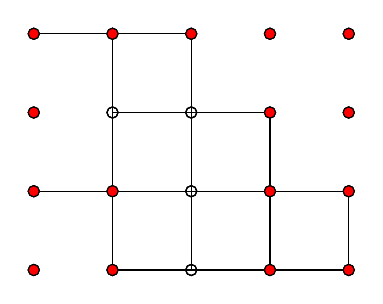
\begin{tikzpicture}[scale=1]%
\path[draw] (1.0,-6.0) -- (1.0,-7.0);%
\path[draw] (1.0,-6.0) -- (2.0,-6.0);%
\path[draw,radius=2pt] (1.0,-6.0) circle;%
\path[draw] (2.0,-6.0) -- (2.0,-7.0);%
\path[draw] (2.0,-6.0) -- (1.0,-6.0);%
\path[draw,radius=2pt] (2.0,-6.0) circle;%
\path[draw] (0.0,-7.0) -- (1.0,-7.0);%
\path[draw,radius=2pt] (0.0,-7.0) circle;%
\path[draw] (1.0,-7.0) -- (1.0,-6.0);%
\path[draw] (1.0,-7.0) -- (1.0,-8.0);%
\path[draw] (1.0,-7.0) -- (0.0,-7.0);%
\path[draw] (1.0,-7.0) -- (2.0,-7.0);%
\path[draw,radius=2pt] (1.0,-7.0) circle;%
\path[draw] (2.0,-7.0) -- (2.0,-6.0);%
\path[draw] (2.0,-7.0) -- (2.0,-8.0);%
\path[draw] (2.0,-7.0) -- (1.0,-7.0);%
\path[draw,radius=2pt] (2.0,-7.0) circle;%
\path[draw] (1.0,-8.0) -- (1.0,-7.0);%
\path[draw] (1.0,-8.0) -- (2.0,-8.0);%
\path[draw,radius=2pt] (1.0,-8.0) circle;%
\path[draw] (2.0,-8.0) -- (2.0,-7.0);%
\path[draw] (2.0,-8.0) -- (1.0,-8.0);%
\path[draw,radius=2pt] (2.0,-8.0) circle;%
\path[draw] (1.0,-6.0) -- (1.0,-7.0);%
\path[draw] (1.0,-6.0) -- (2.0,-6.0);%
\path[draw,radius=2pt] (1.0,-6.0) circle;%
\path[draw] (2.0,-6.0) -- (2.0,-7.0);%
\path[draw] (2.0,-6.0) -- (1.0,-6.0);%
\path[draw,radius=2pt] (2.0,-6.0) circle;%
\path[draw] (1.0,-7.0) -- (1.0,-6.0);%
\path[draw] (1.0,-7.0) -- (2.0,-7.0);%
\path[draw,radius=2pt] (1.0,-7.0) circle;%
\path[draw] (2.0,-7.0) -- (2.0,-6.0);%
\path[draw] (2.0,-7.0) -- (2.0,-8.0);%
\path[draw] (2.0,-7.0) -- (1.0,-7.0);%
\path[draw] (2.0,-7.0) -- (3.0,-7.0);%
\path[draw,radius=2pt] (2.0,-7.0) circle;%
\path[draw] (3.0,-7.0) -- (2.0,-7.0);%
\path[draw] (3.0,-7.0) -- (4.0,-7.0);%
\path[draw,radius=2pt] (3.0,-7.0) circle;%
\path[draw] (4.0,-7.0) -- (4.0,-8.0);%
\path[draw] (4.0,-7.0) -- (3.0,-7.0);%
\path[draw,radius=2pt] (4.0,-7.0) circle;%
\path[draw] (2.0,-8.0) -- (2.0,-7.0);%
\path[draw,radius=2pt] (2.0,-8.0) circle;%
\path[draw] (4.0,-8.0) -- (4.0,-7.0);%
\path[draw,radius=2pt] (4.0,-8.0) circle;%
\path[draw] (0.0,-5.0) -- (1.0,-5.0);%
\path[draw,radius=2pt] (0.0,-5.0) circle;%
\path[draw] (1.0,-5.0) -- (1.0,-6.0);%
\path[draw] (1.0,-5.0) -- (0.0,-5.0);%
\path[draw] (1.0,-5.0) -- (2.0,-5.0);%
\path[draw,radius=2pt] (1.0,-5.0) circle;%
\path[draw] (2.0,-5.0) -- (2.0,-6.0);%
\path[draw] (2.0,-5.0) -- (1.0,-5.0);%
\path[draw,radius=2pt] (2.0,-5.0) circle;%
\path[draw] (1.0,-6.0) -- (1.0,-5.0);%
\path[draw] (1.0,-6.0) -- (2.0,-6.0);%
\path[draw,radius=2pt] (1.0,-6.0) circle;%
\path[draw] (2.0,-6.0) -- (2.0,-5.0);%
\path[draw] (2.0,-6.0) -- (2.0,-7.0);%
\path[draw] (2.0,-6.0) -- (1.0,-6.0);%
\path[draw] (2.0,-6.0) -- (3.0,-6.0);%
\path[draw,radius=2pt] (2.0,-6.0) circle;%
\path[draw] (3.0,-6.0) -- (3.0,-7.0);%
\path[draw] (3.0,-6.0) -- (2.0,-6.0);%
\path[draw,radius=2pt] (3.0,-6.0) circle;%
\path[draw] (2.0,-7.0) -- (2.0,-6.0);%
\path[draw] (2.0,-7.0) -- (2.0,-8.0);%
\path[draw] (2.0,-7.0) -- (3.0,-7.0);%
\path[draw,radius=2pt] (2.0,-7.0) circle;%
\path[draw] (3.0,-7.0) -- (3.0,-6.0);%
\path[draw] (3.0,-7.0) -- (3.0,-8.0);%
\path[draw] (3.0,-7.0) -- (2.0,-7.0);%
\path[draw] (3.0,-7.0) -- (4.0,-7.0);%
\path[draw,radius=2pt] (3.0,-7.0) circle;%
\path[draw] (4.0,-7.0) -- (4.0,-8.0);%
\path[draw] (4.0,-7.0) -- (3.0,-7.0);%
\path[draw,radius=2pt] (4.0,-7.0) circle;%
\path[draw] (2.0,-8.0) -- (2.0,-7.0);%
\path[draw] (2.0,-8.0) -- (3.0,-8.0);%
\path[draw,radius=2pt] (2.0,-8.0) circle;%
\path[draw] (3.0,-8.0) -- (3.0,-7.0);%
\path[draw] (3.0,-8.0) -- (2.0,-8.0);%
\path[draw] (3.0,-8.0) -- (4.0,-8.0);%
\path[draw,radius=2pt] (3.0,-8.0) circle;%
\path[draw] (4.0,-8.0) -- (4.0,-7.0);%
\path[draw] (4.0,-8.0) -- (3.0,-8.0);%
\path[draw,radius=2pt] (4.0,-8.0) circle;%
\path[draw,radius=2pt,fill=red] (0.0,-5.0) circle;%
\path[draw,radius=2pt,fill=red] (1.0,-5.0) circle;%
\path[draw,radius=2pt,fill=red] (2.0,-5.0) circle;%
\path[draw,radius=2pt,fill=red] (3.0,-5.0) circle;%
\path[draw,radius=2pt,fill=red] (4.0,-5.0) circle;%
\path[draw,radius=2pt,fill=red] (0.0,-6.0) circle;%
\path[draw,radius=2pt,fill=red] (3.0,-6.0) circle;%
\path[draw,radius=2pt,fill=red] (4.0,-6.0) circle;%
\path[draw,radius=2pt,fill=red] (3.0,-7.0) circle;%
\path[draw,radius=2pt,fill=red] (4.0,-7.0) circle;%
\path[draw,radius=2pt,fill=red] (0.0,-8.0) circle;%
\path[draw,radius=2pt,fill=red] (3.0,-8.0) circle;%
\path[draw,radius=2pt,fill=red] (4.0,-8.0) circle;%
\path[draw,radius=2pt,fill=red] (0.0,-5.0) circle;%
\path[draw,radius=2pt,fill=red] (1.0,-5.0) circle;%
\path[draw,radius=2pt,fill=red] (2.0,-5.0) circle;%
\path[draw,radius=2pt,fill=red] (3.0,-5.0) circle;%
\path[draw,radius=2pt,fill=red] (4.0,-5.0) circle;%
\path[draw,radius=2pt,fill=red] (0.0,-6.0) circle;%
\path[draw,radius=2pt,fill=red] (3.0,-6.0) circle;%
\path[draw,radius=2pt,fill=red] (4.0,-6.0) circle;%
\path[draw,radius=2pt,fill=red] (0.0,-7.0) circle;%
\path[draw,radius=2pt,fill=red] (0.0,-8.0) circle;%
\path[draw,radius=2pt,fill=red] (1.0,-8.0) circle;%
\path[draw,radius=2pt,fill=red] (3.0,-8.0) circle;%
\path[draw,radius=2pt,fill=red] (3.0,-5.0) circle;%
\path[draw,radius=2pt,fill=red] (4.0,-5.0) circle;%
\path[draw,radius=2pt,fill=red] (0.0,-6.0) circle;%
\path[draw,radius=2pt,fill=red] (4.0,-6.0) circle;%
\path[draw,radius=2pt,fill=red] (0.0,-7.0) circle;%
\path[draw,radius=2pt,fill=red] (1.0,-7.0) circle;%
\path[draw,radius=2pt,fill=red] (0.0,-8.0) circle;%
\path[draw,radius=2pt,fill=red] (1.0,-8.0) circle;%
\end{tikzpicture}%
\hspace*{1in}%
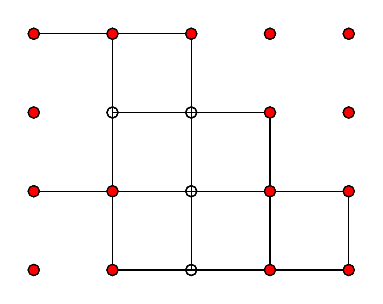
\begin{tikzpicture}[scale=1]%
\path[draw] (1.0,-6.0) -- (1.0,-7.0);%
\path[draw] (1.0,-6.0) -- (2.0,-6.0);%
\path[draw,radius=2pt] (1.0,-6.0) circle;%
\path[draw] (2.0,-6.0) -- (2.0,-7.0);%
\path[draw] (2.0,-6.0) -- (1.0,-6.0);%
\path[draw,radius=2pt] (2.0,-6.0) circle;%
\path[draw] (0.0,-7.0) -- (1.0,-7.0);%
\path[draw,radius=2pt] (0.0,-7.0) circle;%
\path[draw] (1.0,-7.0) -- (1.0,-6.0);%
\path[draw] (1.0,-7.0) -- (1.0,-8.0);%
\path[draw] (1.0,-7.0) -- (0.0,-7.0);%
\path[draw] (1.0,-7.0) -- (2.0,-7.0);%
\path[draw,radius=2pt] (1.0,-7.0) circle;%
\path[draw] (2.0,-7.0) -- (2.0,-6.0);%
\path[draw] (2.0,-7.0) -- (2.0,-8.0);%
\path[draw] (2.0,-7.0) -- (1.0,-7.0);%
\path[draw,radius=2pt] (2.0,-7.0) circle;%
\path[draw] (1.0,-8.0) -- (1.0,-7.0);%
\path[draw] (1.0,-8.0) -- (2.0,-8.0);%
\path[draw,radius=2pt] (1.0,-8.0) circle;%
\path[draw] (2.0,-8.0) -- (2.0,-7.0);%
\path[draw] (2.0,-8.0) -- (1.0,-8.0);%
\path[draw,radius=2pt] (2.0,-8.0) circle;%
\path[draw] (1.0,-6.0) -- (1.0,-7.0);%
\path[draw] (1.0,-6.0) -- (2.0,-6.0);%
\path[draw,radius=2pt] (1.0,-6.0) circle;%
\path[draw] (2.0,-6.0) -- (2.0,-7.0);%
\path[draw] (2.0,-6.0) -- (1.0,-6.0);%
\path[draw] (2.0,-6.0) -- (3.0,-6.0);%
\path[draw,radius=2pt] (2.0,-6.0) circle;%
\path[draw] (3.0,-6.0) -- (3.0,-7.0);%
\path[draw] (3.0,-6.0) -- (2.0,-6.0);%
\path[draw,radius=2pt] (3.0,-6.0) circle;%
\path[draw] (0.0,-7.0) -- (1.0,-7.0);%
\path[draw,radius=2pt] (0.0,-7.0) circle;%
\path[draw] (1.0,-7.0) -- (1.0,-6.0);%
\path[draw] (1.0,-7.0) -- (0.0,-7.0);%
\path[draw] (1.0,-7.0) -- (2.0,-7.0);%
\path[draw,radius=2pt] (1.0,-7.0) circle;%
\path[draw] (2.0,-7.0) -- (2.0,-6.0);%
\path[draw] (2.0,-7.0) -- (2.0,-8.0);%
\path[draw] (2.0,-7.0) -- (1.0,-7.0);%
\path[draw] (2.0,-7.0) -- (3.0,-7.0);%
\path[draw,radius=2pt] (2.0,-7.0) circle;%
\path[draw] (3.0,-7.0) -- (3.0,-6.0);%
\path[draw] (3.0,-7.0) -- (2.0,-7.0);%
\path[draw] (3.0,-7.0) -- (4.0,-7.0);%
\path[draw,radius=2pt] (3.0,-7.0) circle;%
\path[draw] (4.0,-7.0) -- (4.0,-8.0);%
\path[draw] (4.0,-7.0) -- (3.0,-7.0);%
\path[draw,radius=2pt] (4.0,-7.0) circle;%
\path[draw] (2.0,-8.0) -- (2.0,-7.0);%
\path[draw,radius=2pt] (2.0,-8.0) circle;%
\path[draw] (4.0,-8.0) -- (4.0,-7.0);%
\path[draw,radius=2pt] (4.0,-8.0) circle;%
\path[draw] (0.0,-5.0) -- (1.0,-5.0);%
\path[draw,radius=2pt] (0.0,-5.0) circle;%
\path[draw] (1.0,-5.0) -- (1.0,-6.0);%
\path[draw] (1.0,-5.0) -- (0.0,-5.0);%
\path[draw] (1.0,-5.0) -- (2.0,-5.0);%
\path[draw,radius=2pt] (1.0,-5.0) circle;%
\path[draw] (2.0,-5.0) -- (2.0,-6.0);%
\path[draw] (2.0,-5.0) -- (1.0,-5.0);%
\path[draw,radius=2pt] (2.0,-5.0) circle;%
\path[draw] (1.0,-6.0) -- (1.0,-5.0);%
\path[draw] (1.0,-6.0) -- (2.0,-6.0);%
\path[draw,radius=2pt] (1.0,-6.0) circle;%
\path[draw] (2.0,-6.0) -- (2.0,-5.0);%
\path[draw] (2.0,-6.0) -- (2.0,-7.0);%
\path[draw] (2.0,-6.0) -- (1.0,-6.0);%
\path[draw] (2.0,-6.0) -- (3.0,-6.0);%
\path[draw,radius=2pt] (2.0,-6.0) circle;%
\path[draw] (3.0,-6.0) -- (3.0,-7.0);%
\path[draw] (3.0,-6.0) -- (2.0,-6.0);%
\path[draw,radius=2pt] (3.0,-6.0) circle;%
\path[draw] (2.0,-7.0) -- (2.0,-6.0);%
\path[draw] (2.0,-7.0) -- (2.0,-8.0);%
\path[draw] (2.0,-7.0) -- (3.0,-7.0);%
\path[draw,radius=2pt] (2.0,-7.0) circle;%
\path[draw] (3.0,-7.0) -- (3.0,-6.0);%
\path[draw] (3.0,-7.0) -- (3.0,-8.0);%
\path[draw] (3.0,-7.0) -- (2.0,-7.0);%
\path[draw] (3.0,-7.0) -- (4.0,-7.0);%
\path[draw,radius=2pt] (3.0,-7.0) circle;%
\path[draw] (4.0,-7.0) -- (4.0,-8.0);%
\path[draw] (4.0,-7.0) -- (3.0,-7.0);%
\path[draw,radius=2pt] (4.0,-7.0) circle;%
\path[draw] (2.0,-8.0) -- (2.0,-7.0);%
\path[draw] (2.0,-8.0) -- (3.0,-8.0);%
\path[draw,radius=2pt] (2.0,-8.0) circle;%
\path[draw] (3.0,-8.0) -- (3.0,-7.0);%
\path[draw] (3.0,-8.0) -- (2.0,-8.0);%
\path[draw] (3.0,-8.0) -- (4.0,-8.0);%
\path[draw,radius=2pt] (3.0,-8.0) circle;%
\path[draw] (4.0,-8.0) -- (4.0,-7.0);%
\path[draw] (4.0,-8.0) -- (3.0,-8.0);%
\path[draw,radius=2pt] (4.0,-8.0) circle;%
\path[draw,radius=2pt,fill=red] (0.0,-5.0) circle;%
\path[draw,radius=2pt,fill=red] (1.0,-5.0) circle;%
\path[draw,radius=2pt,fill=red] (2.0,-5.0) circle;%
\path[draw,radius=2pt,fill=red] (3.0,-5.0) circle;%
\path[draw,radius=2pt,fill=red] (4.0,-5.0) circle;%
\path[draw,radius=2pt,fill=red] (0.0,-6.0) circle;%
\path[draw,radius=2pt,fill=red] (3.0,-6.0) circle;%
\path[draw,radius=2pt,fill=red] (4.0,-6.0) circle;%
\path[draw,radius=2pt,fill=red] (3.0,-7.0) circle;%
\path[draw,radius=2pt,fill=red] (4.0,-7.0) circle;%
\path[draw,radius=2pt,fill=red] (0.0,-8.0) circle;%
\path[draw,radius=2pt,fill=red] (3.0,-8.0) circle;%
\path[draw,radius=2pt,fill=red] (4.0,-8.0) circle;%
\path[draw,radius=2pt,fill=red] (0.0,-5.0) circle;%
\path[draw,radius=2pt,fill=red] (1.0,-5.0) circle;%
\path[draw,radius=2pt,fill=red] (2.0,-5.0) circle;%
\path[draw,radius=2pt,fill=red] (3.0,-5.0) circle;%
\path[draw,radius=2pt,fill=red] (4.0,-5.0) circle;%
\path[draw,radius=2pt,fill=red] (0.0,-6.0) circle;%
\path[draw,radius=2pt,fill=red] (4.0,-6.0) circle;%
\path[draw,radius=2pt,fill=red] (0.0,-8.0) circle;%
\path[draw,radius=2pt,fill=red] (1.0,-8.0) circle;%
\path[draw,radius=2pt,fill=red] (3.0,-8.0) circle;%
\path[draw,radius=2pt,fill=red] (3.0,-5.0) circle;%
\path[draw,radius=2pt,fill=red] (4.0,-5.0) circle;%
\path[draw,radius=2pt,fill=red] (0.0,-6.0) circle;%
\path[draw,radius=2pt,fill=red] (4.0,-6.0) circle;%
\path[draw,radius=2pt,fill=red] (0.0,-7.0) circle;%
\path[draw,radius=2pt,fill=red] (1.0,-7.0) circle;%
\path[draw,radius=2pt,fill=red] (0.0,-8.0) circle;%
\path[draw,radius=2pt,fill=red] (1.0,-8.0) circle;%
\end{tikzpicture}%
\hspace*{1in}%
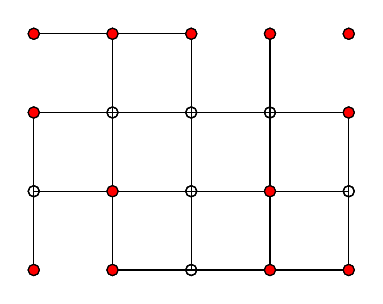
\begin{tikzpicture}[scale=1]%
\path[draw,radius=2pt] (0.0,-5.0) circle;%
\path[draw] (2.0,-5.0) -- (2.0,-6.0);%
\path[draw,radius=2pt] (2.0,-5.0) circle;%
\path[draw,radius=2pt] (4.0,-5.0) circle;%
\path[draw] (1.0,-6.0) -- (1.0,-7.0);%
\path[draw] (1.0,-6.0) -- (2.0,-6.0);%
\path[draw,radius=2pt] (1.0,-6.0) circle;%
\path[draw] (2.0,-6.0) -- (2.0,-5.0);%
\path[draw] (2.0,-6.0) -- (2.0,-7.0);%
\path[draw] (2.0,-6.0) -- (1.0,-6.0);%
\path[draw] (2.0,-6.0) -- (3.0,-6.0);%
\path[draw,radius=2pt] (2.0,-6.0) circle;%
\path[draw] (3.0,-6.0) -- (2.0,-6.0);%
\path[draw,radius=2pt] (3.0,-6.0) circle;%
\path[draw] (0.0,-7.0) -- (1.0,-7.0);%
\path[draw,radius=2pt] (0.0,-7.0) circle;%
\path[draw] (1.0,-7.0) -- (1.0,-6.0);%
\path[draw] (1.0,-7.0) -- (1.0,-8.0);%
\path[draw] (1.0,-7.0) -- (0.0,-7.0);%
\path[draw] (1.0,-7.0) -- (2.0,-7.0);%
\path[draw,radius=2pt] (1.0,-7.0) circle;%
\path[draw] (2.0,-7.0) -- (2.0,-6.0);%
\path[draw] (2.0,-7.0) -- (2.0,-8.0);%
\path[draw] (2.0,-7.0) -- (1.0,-7.0);%
\path[draw,radius=2pt] (2.0,-7.0) circle;%
\path[draw,radius=2pt] (4.0,-7.0) circle;%
\path[draw] (1.0,-8.0) -- (1.0,-7.0);%
\path[draw] (1.0,-8.0) -- (2.0,-8.0);%
\path[draw,radius=2pt] (1.0,-8.0) circle;%
\path[draw] (2.0,-8.0) -- (2.0,-7.0);%
\path[draw] (2.0,-8.0) -- (1.0,-8.0);%
\path[draw] (2.0,-8.0) -- (3.0,-8.0);%
\path[draw,radius=2pt] (2.0,-8.0) circle;%
\path[draw] (3.0,-8.0) -- (2.0,-8.0);%
\path[draw,radius=2pt] (3.0,-8.0) circle;%
\path[draw] (1.0,-5.0) -- (1.0,-6.0);%
\path[draw,radius=2pt] (1.0,-5.0) circle;%
\path[draw] (3.0,-5.0) -- (3.0,-6.0);%
\path[draw,radius=2pt] (3.0,-5.0) circle;%
\path[draw] (0.0,-6.0) -- (0.0,-7.0);%
\path[draw] (0.0,-6.0) -- (1.0,-6.0);%
\path[draw,radius=2pt] (0.0,-6.0) circle;%
\path[draw] (1.0,-6.0) -- (1.0,-5.0);%
\path[draw] (1.0,-6.0) -- (1.0,-7.0);%
\path[draw] (1.0,-6.0) -- (0.0,-6.0);%
\path[draw] (1.0,-6.0) -- (2.0,-6.0);%
\path[draw,radius=2pt] (1.0,-6.0) circle;%
\path[draw] (2.0,-6.0) -- (2.0,-7.0);%
\path[draw] (2.0,-6.0) -- (1.0,-6.0);%
\path[draw] (2.0,-6.0) -- (3.0,-6.0);%
\path[draw,radius=2pt] (2.0,-6.0) circle;%
\path[draw] (3.0,-6.0) -- (3.0,-5.0);%
\path[draw] (3.0,-6.0) -- (3.0,-7.0);%
\path[draw] (3.0,-6.0) -- (2.0,-6.0);%
\path[draw] (3.0,-6.0) -- (4.0,-6.0);%
\path[draw,radius=2pt] (3.0,-6.0) circle;%
\path[draw] (4.0,-6.0) -- (4.0,-7.0);%
\path[draw] (4.0,-6.0) -- (3.0,-6.0);%
\path[draw,radius=2pt] (4.0,-6.0) circle;%
\path[draw] (0.0,-7.0) -- (0.0,-6.0);%
\path[draw] (0.0,-7.0) -- (0.0,-8.0);%
\path[draw] (0.0,-7.0) -- (1.0,-7.0);%
\path[draw,radius=2pt] (0.0,-7.0) circle;%
\path[draw] (1.0,-7.0) -- (1.0,-6.0);%
\path[draw] (1.0,-7.0) -- (0.0,-7.0);%
\path[draw] (1.0,-7.0) -- (2.0,-7.0);%
\path[draw,radius=2pt] (1.0,-7.0) circle;%
\path[draw] (2.0,-7.0) -- (2.0,-6.0);%
\path[draw] (2.0,-7.0) -- (2.0,-8.0);%
\path[draw] (2.0,-7.0) -- (1.0,-7.0);%
\path[draw] (2.0,-7.0) -- (3.0,-7.0);%
\path[draw,radius=2pt] (2.0,-7.0) circle;%
\path[draw] (3.0,-7.0) -- (3.0,-6.0);%
\path[draw] (3.0,-7.0) -- (2.0,-7.0);%
\path[draw] (3.0,-7.0) -- (4.0,-7.0);%
\path[draw,radius=2pt] (3.0,-7.0) circle;%
\path[draw] (4.0,-7.0) -- (4.0,-6.0);%
\path[draw] (4.0,-7.0) -- (4.0,-8.0);%
\path[draw] (4.0,-7.0) -- (3.0,-7.0);%
\path[draw,radius=2pt] (4.0,-7.0) circle;%
\path[draw] (0.0,-8.0) -- (0.0,-7.0);%
\path[draw,radius=2pt] (0.0,-8.0) circle;%
\path[draw] (2.0,-8.0) -- (2.0,-7.0);%
\path[draw,radius=2pt] (2.0,-8.0) circle;%
\path[draw] (4.0,-8.0) -- (4.0,-7.0);%
\path[draw,radius=2pt] (4.0,-8.0) circle;%
\path[draw] (0.0,-5.0) -- (1.0,-5.0);%
\path[draw,radius=2pt] (0.0,-5.0) circle;%
\path[draw] (1.0,-5.0) -- (1.0,-6.0);%
\path[draw] (1.0,-5.0) -- (0.0,-5.0);%
\path[draw] (1.0,-5.0) -- (2.0,-5.0);%
\path[draw,radius=2pt] (1.0,-5.0) circle;%
\path[draw] (2.0,-5.0) -- (2.0,-6.0);%
\path[draw] (2.0,-5.0) -- (1.0,-5.0);%
\path[draw,radius=2pt] (2.0,-5.0) circle;%
\path[draw,radius=2pt] (4.0,-5.0) circle;%
\path[draw] (1.0,-6.0) -- (1.0,-5.0);%
\path[draw] (1.0,-6.0) -- (2.0,-6.0);%
\path[draw,radius=2pt] (1.0,-6.0) circle;%
\path[draw] (2.0,-6.0) -- (2.0,-5.0);%
\path[draw] (2.0,-6.0) -- (2.0,-7.0);%
\path[draw] (2.0,-6.0) -- (1.0,-6.0);%
\path[draw] (2.0,-6.0) -- (3.0,-6.0);%
\path[draw,radius=2pt] (2.0,-6.0) circle;%
\path[draw] (3.0,-6.0) -- (3.0,-7.0);%
\path[draw] (3.0,-6.0) -- (2.0,-6.0);%
\path[draw,radius=2pt] (3.0,-6.0) circle;%
\path[draw,radius=2pt] (0.0,-7.0) circle;%
\path[draw] (2.0,-7.0) -- (2.0,-6.0);%
\path[draw] (2.0,-7.0) -- (2.0,-8.0);%
\path[draw] (2.0,-7.0) -- (3.0,-7.0);%
\path[draw,radius=2pt] (2.0,-7.0) circle;%
\path[draw] (3.0,-7.0) -- (3.0,-6.0);%
\path[draw] (3.0,-7.0) -- (3.0,-8.0);%
\path[draw] (3.0,-7.0) -- (2.0,-7.0);%
\path[draw] (3.0,-7.0) -- (4.0,-7.0);%
\path[draw,radius=2pt] (3.0,-7.0) circle;%
\path[draw] (4.0,-7.0) -- (4.0,-8.0);%
\path[draw] (4.0,-7.0) -- (3.0,-7.0);%
\path[draw,radius=2pt] (4.0,-7.0) circle;%
\path[draw] (1.0,-8.0) -- (2.0,-8.0);%
\path[draw,radius=2pt] (1.0,-8.0) circle;%
\path[draw] (2.0,-8.0) -- (2.0,-7.0);%
\path[draw] (2.0,-8.0) -- (1.0,-8.0);%
\path[draw] (2.0,-8.0) -- (3.0,-8.0);%
\path[draw,radius=2pt] (2.0,-8.0) circle;%
\path[draw] (3.0,-8.0) -- (3.0,-7.0);%
\path[draw] (3.0,-8.0) -- (2.0,-8.0);%
\path[draw] (3.0,-8.0) -- (4.0,-8.0);%
\path[draw,radius=2pt] (3.0,-8.0) circle;%
\path[draw] (4.0,-8.0) -- (4.0,-7.0);%
\path[draw] (4.0,-8.0) -- (3.0,-8.0);%
\path[draw,radius=2pt] (4.0,-8.0) circle;%
\path[draw,radius=2pt,fill=red] (1.0,-5.0) circle;%
\path[draw,radius=2pt,fill=red] (3.0,-5.0) circle;%
\path[draw,radius=2pt,fill=red] (0.0,-6.0) circle;%
\path[draw,radius=2pt,fill=red] (4.0,-6.0) circle;%
\path[draw,radius=2pt,fill=red] (3.0,-7.0) circle;%
\path[draw,radius=2pt,fill=red] (0.0,-8.0) circle;%
\path[draw,radius=2pt,fill=red] (4.0,-8.0) circle;%
\path[draw,radius=2pt,fill=red] (0.0,-5.0) circle;%
\path[draw,radius=2pt,fill=red] (2.0,-5.0) circle;%
\path[draw,radius=2pt,fill=red] (4.0,-5.0) circle;%
\path[draw,radius=2pt,fill=red] (1.0,-8.0) circle;%
\path[draw,radius=2pt,fill=red] (3.0,-8.0) circle;%
\path[draw,radius=2pt,fill=red] (3.0,-5.0) circle;%
\path[draw,radius=2pt,fill=red] (0.0,-6.0) circle;%
\path[draw,radius=2pt,fill=red] (4.0,-6.0) circle;%
\path[draw,radius=2pt,fill=red] (1.0,-7.0) circle;%
\path[draw,radius=2pt,fill=red] (0.0,-8.0) circle;%
\end{tikzpicture}%
\end{document}